\documentclass[11pt, oneside]{article}   	% use "amsart" instead of "article" for AMSLaTeX format
\usepackage{geometry}                		% See geometry.pdf to learn the layout options. There are lots.
\geometry{letterpaper}                   		% ... or a4paper or a5paper or ... 
%\geometry{landscape}                		% Activate for for rotated page geometry
%\usepackage[parfill]{parskip}    		% Activate to begin paragraphs with an empty line rather than an indent
\usepackage{graphicx}				% Use pdf, png, jpg, or eps§ with pdflatex; use eps in DVI mode
								% TeX will automatically convert eps --> pdf in pdflatex
\usepackage{amssymb}


\title{SE 464 Prototype Demo -- Shots Fired}
\author{Sam Maier (scmaier), Addison Keizer (wcakeize), \\Dhruv Lal (d2lal), Shiranka Miskin (samiskin)}
%\date{}							% Activate to display a given date or no date
\let\endtitlepage\relax
\begin{document}
\maketitle


\clearpage

\section{Demo Summary}
\hspace*{5mm}In this demo, we demonstrate an instance of our second user scenario. The user
is presented with a splash screen containing a button to start ``Quick Play".
This is the mode that will be used for people that are not playing with a group
of friends. When clicked, the user will be taken to a loading screen.
Once there is at least 2 people and a time limit is
reached or four people have joined, the game will start and each user will have
a character on the map. The user can move their character using the arrow keys,
aim the character's gun using the mouse pointer, and shoot using a left-click
on the mouse. Each player will have a fixed amount of health and when they get
shot, they will lose one health. After a character loses all of their health,
they die and the game is over.

\section{Status Report}
\hspace*{5mm}
Currently, we have the functionality of the actual character game play completed. There
is a basic splash screen at the moment with an option to ``Quick Play". This is
used for the user to join a game without friends. The functionality for joining
a non-friend game is complete such that a game starts when there are at least
two people and a time limit has been reached, or four people have joined.\\

In addition to this, we need to create a button to ``Play with Friends". Within
this, a user would be able to create a private group. Users will be able to
join this private group by entering a URL or entering a code within the ``Play
with Friends" option.\\

Within the gameplay, when there is only one player left, the game is over, and an appropriate screen
will have to be displayed for the user indicating that the user has won or that
the game is over. From there, there will be a button that will take the user
back to the main menu / splash screen. If it is a game with a group of friends,
there will be an option to play another game with the some people.\\

In terms of difficulties we've encountered, they have been server related issues.
Right now, unless the server is funning at 60 FPS, the player movement of non-user controlled characters will be choppy and delayed.
This will have to be improved so that all player movement is smooth.
We are also experiencing some syncing issues between the client and server.
In the prototype demo, the server runs at such a speed that this is not noticeable,
however we will need to do something to fix these issues so that there is no delay in events and actions between the client(s) and server.

\clearpage

\section{Architecture Overview}

MVC Architecture:\\
\begin{center}
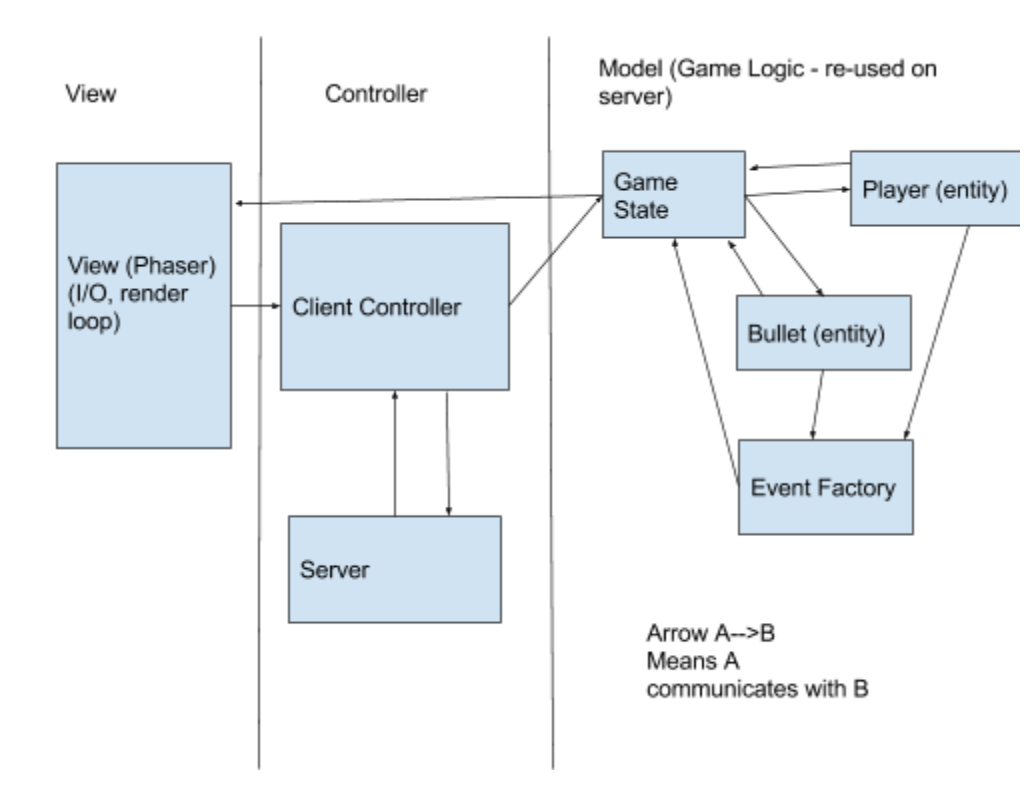
\includegraphics[scale=0.7]{images/mvc-architecture.png}
\end{center}

Entity Hierarchy:\\
\begin{center}
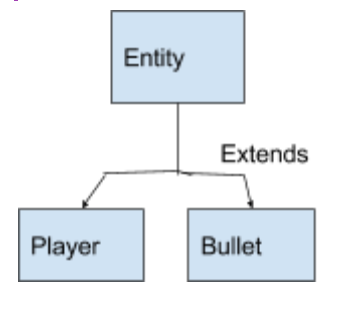
\includegraphics[scale=0.9]{images/entity-hierarchy.png}
\end{center}
In our system, we have two different entities representing objects that can be seen on screen.\\

\clearpage

Client / Server Architecture:\\
\begin{center}
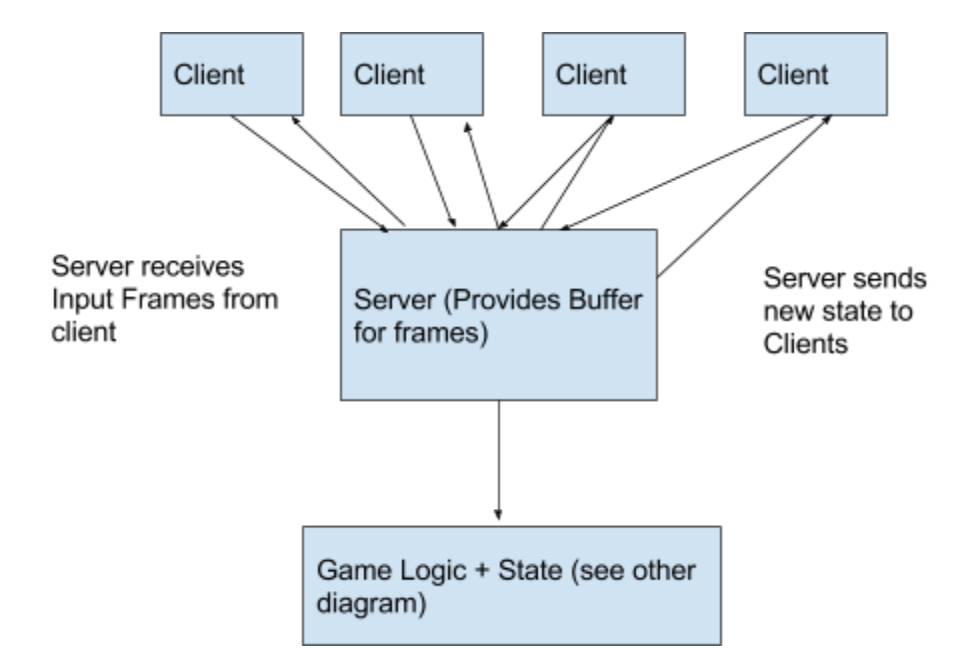
\includegraphics[scale=0.7]{images/client-server-architecture.png}
\end{center}



\end{document}
